\documentclass[12pt,a4paper]{article}

\usepackage{iftex}
\ifPDFTeX
  \usepackage[utf8]{inputenc}
  \usepackage[T2A]{fontenc}
\else
  \usepackage{fontspec}
  \setmainfont{cmunrm.otf}[Path=docs/fonts/,BoldFont=cmunbx.otf,ItalicFont=cmunti.otf,BoldItalicFont=cmunbi.otf]
  \setmonofont{cmuntt.otf}[Path=docs/fonts/,BoldFont=cmuntb.otf,ItalicFont=cmunit.otf,BoldItalicFont=cmuntx.otf]
\fi
\usepackage[russian]{babel}
\usepackage{amsmath}
\usepackage{amssymb}
\usepackage{array}
\usepackage{booktabs}
\usepackage{caption}
\usepackage{enumitem}
\usepackage{fancyhdr}
\usepackage{float}
\usepackage{geometry}
\usepackage{graphicx}
\usepackage{hyperref}
\usepackage{indentfirst}
\usepackage{listings}
\usepackage{longtable}
\usepackage{tikz}
\usepackage{xcolor}
\usetikzlibrary{arrows.meta,positioning,shapes.geometric}

\geometry{left=30mm,right=15mm,top=20mm,bottom=20mm}
\setlength{\parindent}{1.25cm}
\linespread{1.2}
\pagestyle{fancy}
\fancyhf{}
\fancyfoot[C]{\thepage}
\renewcommand{\headrulewidth}{0pt}
\hypersetup{hidelinks}

\captionsetup{justification=centering}
\setcounter{tocdepth}{2}

\definecolor{codebg}{RGB}{248,248,248}
\definecolor{codeframe}{RGB}{215,215,215}
\definecolor{codekw}{RGB}{0,76,153}
\definecolor{codestr}{RGB}{163,21,21}
\definecolor{codecomment}{RGB}{0,128,0}

\lstdefinelanguage{JavaScript}{
  morekeywords={const,let,var,function,return,if,else,for,while,throw,new,export,import,from,class,get},
  sensitive=true,
  morecomment=[l]{//},
  morestring=[b]",
  morestring=[b]',
}

\lstset{
  language=JavaScript,
  basicstyle=\ttfamily\small,
  keywordstyle=\color{codekw}\bfseries,
  stringstyle=\color{codestr},
  commentstyle=\color{codecomment},
  backgroundcolor=\color{codebg},
  frame=single,
  rulecolor=\color{codeframe},
  numbers=left,
  numberstyle=\tiny,
  stepnumber=1,
  breaklines=true,
  showstringspaces=false,
  tabsize=2,
  columns=fullflexible,
  keepspaces=true,
  extendedchars=true,
  inputencoding=utf8
}

\newcolumntype{C}[1]{>{\centering\arraybackslash}p{#1}}

\begin{document}

% ====================== ТИТУЛЬНЫЙ ЛИСТ ======================
\pagenumbering{gobble}
\hypersetup{pageanchor=false}
\begin{titlepage}
  \thispagestyle{empty}
  \begin{center}
    {\small Федеральное государственное автономное образовательное учреждение высшего образования\\
    «Национальный исследовательский университет ИТМО»}\\[0.8em]
    {\small Факультет программной инженерии и компьютерной техники}

    \vfill

    {\Large\textbf{Лабораторная работа №5}}\\[0.6em]
    {\large по курсу «Вычислительная математика»}\\[0.6em]
    {\large Вариант 19}

    \vfill

    \begin{flushright}
      \begin{tabular}{l}
        Выполнил:\\
        Якименко Владислав Игоревич, Р3213\\[0.8em]
        Проверила:\\
        Малышева Татьяна Алексеевна
      \end{tabular}
    \end{flushright}

    \vfill

    Санкт-Петербург --- 2026
  \end{center}
\end{titlepage}
\clearpage
\hypersetup{pageanchor=true}

\tableofcontents
\thispagestyle{empty}
\clearpage
\pagenumbering{arabic}


% CONTENT
\section{Вычислительная реализация задачи}
\subsection{Постановка задачи}
\textbf{Цель работы:} решить задачу интерполяции и найти значения функции
при аргументах, отличных от узловых точек; сравнить результаты различных
представлений интерполяционного многочлена.

\textbf{Порядок выполнения работы:}
\begin{enumerate}[label=\arabic*.,leftmargin=1.2cm]
\item Выбрать таблицу 1.4 для варианта 19 и построить таблицу конечных разностей.
\item Вычислить $f(X_1)$ подходящей формулой Ньютона, а $f(X_2)$ --- формулой Гаусса.
\item Для обоих аргументов выполнить проверку многочленом Лагранжа.
\item Реализовать ввод данных, расчёт разностей, сравнение методов и графики; проверить корректные и ошибочные наборы.
\end{enumerate}
\[
X_1=1.573,\qquad X_2=1.375,\qquad h=0.1.
\]
\begin{table}[H]\centering
\caption{Исходные данные варианта 19 (таблица 1.4 задания)}
\begin{tabular}{c*{7}{r}}\toprule
$x_i$ & 1.05 & 1.15 & 1.25 & 1.35 & 1.45 & 1.55 & 1.65\\
$y_i$ & 0.1213 & 1.1316 & 2.1459 & 3.1565 & 4.1571 & 5.1819 & 6.1969\\\bottomrule
\end{tabular}\end{table}

\subsection{Графическое представление}
Аналитическая исходная функция в задании не дана. Поэтому исходные табличные
значения соединены оранжевой пунктирной линией, а полином Ньютона показан
синей линией. Узлы отмечены отдельными точками.

\begin{figure}[H]\centering

\includegraphics[width=0.88\textwidth]{docs/graph-computational.png}
\caption{Табличные данные, полином Ньютона, узлы и точка $X_1=1.573$}
\end{figure}

\clearpage
\subsection{Рабочие формулы метода}
Пусть заданы $n+1$ различных узлов $(x_i,y_i)$, $i=0,\ldots,n$.
Ищем полином $P_n$ степени не выше $n$, удовлетворяющий условию
$P_n(x_i)=y_i$. В данной работе $n=6$.

\textbf{Многочлен Лагранжа:}
\[
 L_n(x)=\sum_{i=0}^{n}y_i\ell_i(x),\qquad
 \ell_i(x)=\prod_{\substack{j=0\\j\ne i}}^{n}\frac{x-x_j}{x_i-x_j}.
\]
\textbf{Разделённые разности:}
\[
 f[x_i]=y_i,\qquad
 f[x_i,\ldots,x_{i+k}]=\frac{f[x_{i+1},\ldots,x_{i+k}]-f[x_i,\ldots,x_{i+k-1}]}{x_{i+k}-x_i}.
\]
\textbf{Ньютон с разделёнными разностями (I и II):}
\begin{align*}
N_n^{\mathrm I}(x)&=y_0+\sum_{k=1}^{n}f[x_0,\ldots,x_k]\prod_{j=0}^{k-1}(x-x_j),\\
N_n^{\mathrm {II}}(x)&=y_n+\sum_{k=1}^{n}f[x_{n-k},\ldots,x_n]\prod_{j=0}^{k-1}(x-x_{n-j}).
\end{align*}
Эти формулы применимы и на неравномерной сетке. Первая удобна в левой
части таблицы, вторая --- в правой.

\textbf{Конечные разности на равномерной сетке:}
\[
\Delta^0 y_i=y_i,\qquad \Delta^k y_i=\Delta^{k-1}y_{i+1}-\Delta^{k-1}y_i.
\]
\textbf{Первая формула Ньютона (вперёд):}
\[
N_n^{\mathrm I}(x)=y_0+\sum_{k=1}^{n}\frac{t(t-1)\cdots(t-k+1)}{k!}\Delta^k y_0,
\qquad t=\frac{x-x_0}{h}.
\]
\textbf{Вторая формула Ньютона (назад):}
\[
N_n^{\mathrm {II}}(x)=y_n+\sum_{k=1}^{n}\frac{t(t+1)\cdots(t+k-1)}{k!}\Delta^k y_{n-k},
\qquad t=\frac{x-x_n}{h}.
\]
При достаточной гладкости исходной функции остаток интерполяции имеет вид
\[
f(x)-P_n(x)=\frac{f^{(n+1)}(\xi)}{(n+1)!}\prod_{i=0}^{n}(x-x_i).
\]
Для табличного варианта производная $f^{(7)}$ неизвестна, поэтому численную
оценку истинной погрешности по этой формуле получить нельзя.

\clearpage
\subsection{Таблица конечных разностей}
Например,
\[
\Delta y_0=1.1316-0.1213=1.0103,
\]
\[
\Delta^2y_0=1.0143-1.0103=0.0040,
\quad \Delta^3y_0=-0.0037-0.0040=-0.0077.
\]
\begin{table}[H]
\centering
\small
\caption{Таблица конечных разностей до шестого порядка}
\begin{tabular}{rrrrrrrr}
\toprule
$x_i$ & $y_i$ & $\Delta^1y_i$ & $\Delta^2y_i$ & $\Delta^3y_i$ & $\Delta^4y_i$ & $\Delta^5y_i$ & $\Delta^6y_i$ \\
\midrule
1.05 & 0.1213 & 1.0103 & 0.0040 & -0.0077 & 0.0014 & 0.0391 & -0.1478 \\
1.15 & 1.1316 & 1.0143 & -0.0037 & -0.0063 & 0.0405 & -0.1087 &  \\
1.25 & 2.1459 & 1.0106 & -0.0100 & 0.0342 & -0.0682 &  &  \\
1.35 & 3.1565 & 1.0006 & 0.0242 & -0.0340 &  &  &  \\
1.45 & 4.1571 & 1.0248 & -0.0098 &  &  &  &  \\
1.55 & 5.1819 & 1.0150 &  &  &  &  &  \\
1.65 & 6.1969 &  &  &  &  &  &  \\
\bottomrule
\end{tabular}
\end{table}

Разности рассчитаны до шестого порядка без промежуточного округления.
Разность шестого порядка ненулевая, поэтому для использования всех исходных
данных сохраняем полином шестой степени.

\subsection{Вычисление $f(X_1)$ по второй формуле Ньютона}
Аргумент $X_1=1.573$ находится в правой половине таблицы и близок к её
правому концу $x_6=1.65$. Используем интерполирование назад:
\[
t=\frac{1.573-1.65}{0.1}=-0.77.
\]
\begin{align*}
N_6^{\mathrm{II}}(x)={}&y_6+t\Delta y_5+\frac{t(t+1)}{2!}\Delta^2y_4
 +\frac{t(t+1)(t+2)}{3!}\Delta^3y_3\\
&+\frac{t(t+1)(t+2)(t+3)}{4!}\Delta^4y_2\\
&+\frac{t(t+1)(t+2)(t+3)(t+4)}{5!}\Delta^5y_1\\
&+\frac{t(t+1)(t+2)(t+3)(t+4)(t+5)}{6!}\Delta^6y_0.
\end{align*}
Из таблицы берём разности $1.0150$, $-0.0098$, $-0.0340$, $-0.0682$,
$-0.1087$, $-0.1478$. Первые два ненулевых слагаемых:
\[
(-0.77)\cdot1.0150=-0.78155,
\qquad \frac{(-0.77)\cdot0.23}{2}\cdot(-0.0098)=0.00086779.
\]
\begin{table}[H]
\centering
\small
\caption{Подстановка $t=-0.77$ во вторую формулу Ньютона}
\begin{tabular}{rrrr}
\toprule
$k$ & Коэффициент & Разность & Слагаемое \\
\midrule
0 & 1 & 6.1969 & 6.196900000000 \\
1 & -0.7700000000 & 1.0150 & -0.781550000000 \\
2 & -0.0885500000 & -0.0098 & 0.000867790000 \\
3 & -0.0363055000 & -0.0340 & 0.001234387000 \\
4 & -0.0202403163 & -0.0682 & 0.001380389568 \\
5 & -0.0130752443 & -0.1087 & 0.001421279055 \\
6 & -0.0092180472 & -0.1478 & 0.001362427381 \\
\bottomrule
\end{tabular}
\end{table}

Суммируя все семь слагаемых, получаем
\[
\boxed{f(1.573)\approx N_6^{\mathrm{II}}(1.573)=5.421616273004}.
\]

\clearpage
\subsection{Вычисление $f(X_2)$ по первой формуле Гаусса}
Центральный узел $a=x_3=1.35$. Здесь удобно переобозначить узлы:
$z_j=x_{j+3}$, $v_j=y_{j+3}$, $j=-3,\ldots,3$.
Тогда $z_0=a$, $v_0=3.1565$, а
\[
X_2=1.375>a,\qquad t=\frac{1.375-1.35}{0.1}=0.25.
\]
Следовательно, используем \textbf{первую формулу Гаусса}:
\begin{align*}
G_6^{\mathrm I}(x)={}&v_0+t\Delta v_0+\frac{t(t-1)}{2!}\Delta^2v_{-1}
 +\frac{t(t-1)(t+1)}{3!}\Delta^3v_{-1}\\
&+\frac{t(t-1)(t+1)(t-2)}{4!}\Delta^4v_{-2}\\
&+\frac{t(t-1)(t+1)(t-2)(t+2)}{5!}\Delta^5v_{-2}\\
&+\frac{t(t-1)(t+1)(t-2)(t+2)(t-3)}{6!}\Delta^6v_{-3}.
\end{align*}
Порядок добавления узлов: $z_0,z_1,z_{-1},z_2,z_{-2},z_3,z_{-3}$.
Из исходной таблицы нужны
\[
\Delta y_3=1.0006,\quad \Delta^2y_2=-0.0100,\quad \Delta^3y_2=0.0342,
\]
\[
\Delta^4y_1=0.0405,\quad \Delta^5y_1=-0.1087,\quad \Delta^6y_0=-0.1478.
\]
Например,
\[
\frac{0.25(-0.75)}{2}(-0.01)=0.0009375,
\]
\[
\frac{0.25(-0.75)(1.25)}{6}(0.0342)=-0.0013359375.
\]
\begin{table}[H]
\centering
\small
\caption{Подстановка $t=0.25$ в первую формулу Гаусса}
\begin{tabular}{rrrr}
\toprule
$k$ & Коэффициент & Разность & Слагаемое \\
\midrule
0 & 1 & 3.1565 & 3.156500000000 \\
1 & 0.2500000000 & 1.0006 & 0.250150000000 \\
2 & -0.0937500000 & -0.0100 & 0.000937500000 \\
3 & -0.0390625000 & 0.0342 & -0.001335937500 \\
4 & 0.0170898438 & 0.0405 & 0.000692138672 \\
5 & 0.0076904297 & -0.1087 & -0.000835949707 \\
6 & -0.0035247803 & -0.1478 & 0.000520962524 \\
\bottomrule
\end{tabular}
\end{table}

Сумма слагаемых:
\[
\boxed{f(1.375)\approx G_6^{\mathrm I}(1.375)=3.406628713989}.
\]

\clearpage
\subsection{Проверка многочленом Лагранжа}
Для равномерной сетки вводим $s=(x-1.05)/0.1$, тогда
\[
\ell_i(x)=\frac{\prod_{j\ne i}(s-j)}{\prod_{j\ne i}(i-j)},
\qquad \prod_{j\ne i}(i-j)=(-1)^{6-i}i!(6-i)!.
\]
Знаменатели для $i=0,\ldots,6$: $720,-120,48,-36,48,-120,720$.
При $X_1$ получаем $s_1=5.23$, при $X_2$ --- $s_2=3.25$.
Например, для центрального базиса в точке $X_2$:
\[
\ell_3(1.375)=\frac{3.25\cdot2.25\cdot1.25\cdot(-0.75)\cdot(-1.75)\cdot(-2.75)}{-36}
=0.916442871094.
\]
\begin{table}[H]
\centering
\caption{Слагаемые многочлена Лагранжа при $x=1.573$}
\begin{tabular}{rrr}
\toprule
$i$ & $\ell_i(x)$ & $y_i\ell_i(x)$ \\
\midrule
0 & -0.009218047230 & -0.001118149129 \\
1 & 0.068383527676 & 0.077382799918 \\
2 & -0.223887246184 & -0.480439641585 \\
3 & 0.432380152570 & 1.364807951586 \\
4 & -0.587931548921 & -2.444090242020 \\
5 & 1.257662269866 & 6.517080116218 \\
6 & 0.062610892223 & 0.387993438015 \\
\bottomrule
\end{tabular}
\end{table}

\begin{table}[H]
\centering
\caption{Слагаемые многочлена Лагранжа при $x=1.375$}
\begin{tabular}{rrr}
\toprule
$i$ & $\ell_i(x)$ & $y_i\ell_i(x)$ \\
\midrule
0 & -0.003524780273 & -0.000427555847 \\
1 & 0.030548095703 & 0.034568225098 \\
2 & -0.137466430664 & -0.294989213562 \\
3 & 0.916442871094 & 2.892751922607 \\
4 & 0.229110717773 & 0.952436164856 \\
5 & -0.039276123047 & -0.203524942017 \\
6 & 0.004165649414 & 0.025814112854 \\
\bottomrule
\end{tabular}
\end{table}

В каждой таблице $\sum_i\ell_i(x)=1$; сумма последнего столбца даёт
\[
\boxed{L_6(1.573)=5.421616273004},\qquad
\boxed{L_6(1.375)=3.406628713989}.
\]
Результаты совпали с выбранными формулами Ньютона и Гаусса. В таблицах
отображены округлённые числа; суммирование выполнялось до округления.

\clearpage
\section{Программная реализация}
Проект написан на JavaScript и запускается в Node.js 20 или новее.
Консоль и браузер используют общий модуль \texttt{src/interpolation.js}.
Внешние библиотеки для интерполяции не используются.

\subsection{Методы, ввод и порядок работы}
Согласно таблице 2 задания для варианта 19 реализованы методы 1, 2, 3:
Лагранж, Ньютон с разделёнными разностями (I и II) и Ньютон с конечными
разностями (I и II). Для проверки вычислительной части добавлены обе
формулы Гаусса. Выполнено также необязательное задание: схемы Стирлинга и Бесселя.

Предусмотрены три способа задания исходных данных:
\begin{enumerate}[leftmargin=1.2cm]
\item Ввод пар $(x,y)$ с клавиатуры в консоли или редактирование таблицы в браузере.
\item Загрузка JSON (\texttt{points} либо массивы \texttt{x}, \texttt{y}) или
текстового файла с двумя числами в строке. Разделители --- пробел и точка с запятой;
допускается десятичная запятая.
\item Табулирование одной из функций $\sin x$, $e^x$, $x^3-2x+1$:
пользователь выбирает интервал, число точек и аргумент интерполяции.
\end{enumerate}

Узлы сортируются по $x$ с сохранением пар $(x,y)$. Проверяются число точек
(от 2 до 50), конечность значений, отсутствие совпадающих или машинно
неразличимых абсцисс и равномерность сетки. Ограничение 50 узлов принято в
реализации, а не перенесено из задания. Неравномерная сетка допустима для
Лагранжа и Ньютона с разделёнными разностями; остальные методы получают
диагностику неприменимости.

Программа выводит обе таблицы разностей на равномерной сетке,
результат каждого метода, рекомендуемое направление Ньютона и максимальное
расхождение применимых методов. Если выбрана известная функция, дополнительно
вычисляется $|P(x)-f(x)|$. Выход за интервал помечается как экстраполяция;
для большой степени полинома выводится предупреждение о численной неустойчивости.

\begin{figure}[H]\centering
\begin{tikzpicture}[node distance=0.5cm,>=Stealth,
block/.style={draw=black!55,align=center,minimum width=12cm,minimum height=0.75cm,inner sep=4pt}]
\node[block] (a) {Выбор источника: клавиатура, файл или функция};
\node[block,below=of a] (b) {Проверка узлов, сортировка, определение шага};
\node[block,below=of b] (c) {Таблицы разностей и проверка применимости методов};
\node[block,below=of c] (d) {Вычисление полиномов в заданной точке и сравнение};
\node[block,below=of d] (e) {Вывод результатов, графика и диагностических сообщений};
\draw[->] (a)--(b);\draw[->] (b)--(c);\draw[->] (c)--(d);\draw[->] (d)--(e);
\end{tikzpicture}
\caption{Основные этапы алгоритма интерполяции}
\end{figure}

\clearpage
\subsection{Дополнительные центральные схемы}
В данной реализации центральные формулы используют полный набор узлов.
Гаусс и Стирлинг реализованы для нечётного числа равноотстоящих узлов,
Бессель --- для чётного. Программа не отбрасывает крайние узлы незаметно
для пользователя, поэтому на семи узлах варианта 19 Бессель помечается как
неприменимый. Его проверка выполняется отдельно на шести узлах.

Для второй формулы Гаусса порядок узлов:
$z_0,z_{-1},z_1,z_{-2},z_2,\ldots$.
Первые слагаемые имеют вид
\[
G^{\mathrm{II}}(x)=v_0+t\Delta v_{-1}
+\frac{t(t+1)}{2!}\Delta^2v_{-1}
+\frac{t(t+1)(t-1)}{3!}\Delta^3v_{-2}+\cdots.
\]
Её обычно выбирают при $x<a$. В точной арифметике обе полные схемы Гаусса
задают тот же полином, что и Лагранж.

\textbf{Стирлинг.} Для $2m+1$ узлов $z_{-m},\ldots,z_m$,
$t=(x-z_0)/h$ и $A_r(t)=\prod_{j=1}^{r-1}(t^2-j^2)$:
\begin{align*}
S_{2m}(x)=v_0+\sum_{r=1}^{m}\bigg[&
\frac{tA_r(t)}{(2r-1)!}\frac{\Delta^{2r-1}v_{-r}+\Delta^{2r-1}v_{-r+1}}{2}\\
&+\frac{t^2A_r(t)}{(2r)!}\Delta^{2r}v_{-r}\bigg].
\end{align*}
Формула является средним двух формул Гаусса; рекомендуется при
$|t|\le0.25$. В чётных слагаемых стоит $t^2$, что также следует из симметрии.
Для $X_2$ получаем $t=0.25$ и $S_6(X_2)=3.406628713989$.

\textbf{Бессель.} Для $2m+2$ узлов $z_{-m},\ldots,z_{m+1}$,
$t=(x-z_0)/h$ и $B_r(t)=\prod_{j=0}^{r-1}(t+j)(t-j-1)$:
\begin{align*}
B_{2m+1}(x)={}&\frac{v_0+v_1}{2}+(t-\tfrac12)\Delta v_0\\
&+\sum_{r=1}^{m}\bigg[\frac{B_r(t)}{(2r)!}
\frac{\Delta^{2r}v_{-r}+\Delta^{2r}v_{-r+1}}{2}\\
&\hspace{3.8cm}+\frac{(t-\tfrac12)B_r(t)}{(2r+1)!}\Delta^{2r+1}v_{-r}\bigg].
\end{align*}
Рекомендуется $0.25\le t\le0.75$. Для проверки использована функция
$f(x)=x^3-2x+1$ на шести узлах:
\[
-1,\quad -0.5,\quad 0,\quad 0.5,\quad 1,\quad 1.5.
\]
Центральная пара --- $0,0.5$.
При $x=0.25$, $t=0.5$ схема Бесселя даёт $0.515625$, что совпадает с $f(0.25)$.

\clearpage
\subsection{Листинг программы}
Ниже приведён расчётный модуль целиком: исходные данные, проверка входа,
таблицы разностей, все методы, табулирование и сравнение результатов.
Остальные файлы проекта содержат консольный ввод, загрузку файлов,
генерацию SVG и веб-интерфейс.

\lstset{literate=
{А}{{\selectfont А}}1
{Б}{{\selectfont Б}}1
{В}{{\selectfont В}}1
{Г}{{\selectfont Г}}1
{Д}{{\selectfont Д}}1
{Е}{{\selectfont Е}}1
{Ё}{{\selectfont Ё}}1
{Ж}{{\selectfont Ж}}1
{З}{{\selectfont З}}1
{И}{{\selectfont И}}1
{Й}{{\selectfont Й}}1
{К}{{\selectfont К}}1
{Л}{{\selectfont Л}}1
{М}{{\selectfont М}}1
{Н}{{\selectfont Н}}1
{О}{{\selectfont О}}1
{П}{{\selectfont П}}1
{Р}{{\selectfont Р}}1
{С}{{\selectfont С}}1
{Т}{{\selectfont Т}}1
{У}{{\selectfont У}}1
{Ф}{{\selectfont Ф}}1
{Х}{{\selectfont Х}}1
{Ц}{{\selectfont Ц}}1
{Ч}{{\selectfont Ч}}1
{Ш}{{\selectfont Ш}}1
{Щ}{{\selectfont Щ}}1
{Ъ}{{\selectfont Ъ}}1
{Ы}{{\selectfont Ы}}1
{Ь}{{\selectfont Ь}}1
{Э}{{\selectfont Э}}1
{Ю}{{\selectfont Ю}}1
{Я}{{\selectfont Я}}1
{а}{{\selectfont а}}1
{б}{{\selectfont б}}1
{в}{{\selectfont в}}1
{г}{{\selectfont г}}1
{д}{{\selectfont д}}1
{е}{{\selectfont е}}1
{ё}{{\selectfont ё}}1
{ж}{{\selectfont ж}}1
{з}{{\selectfont з}}1
{и}{{\selectfont и}}1
{й}{{\selectfont й}}1
{к}{{\selectfont к}}1
{л}{{\selectfont л}}1
{м}{{\selectfont м}}1
{н}{{\selectfont н}}1
{о}{{\selectfont о}}1
{п}{{\selectfont п}}1
{р}{{\selectfont р}}1
{с}{{\selectfont с}}1
{т}{{\selectfont т}}1
{у}{{\selectfont у}}1
{ф}{{\selectfont ф}}1
{х}{{\selectfont х}}1
{ц}{{\selectfont ц}}1
{ч}{{\selectfont ч}}1
{ш}{{\selectfont ш}}1
{щ}{{\selectfont щ}}1
{ъ}{{\selectfont ъ}}1
{ы}{{\selectfont ы}}1
{ь}{{\selectfont ь}}1
{э}{{\selectfont э}}1
{ю}{{\selectfont ю}}1
{я}{{\selectfont я}}1
{≥}{{$\ge$}}1 {≤}{{$\le$}}1 {−}{{$-$}}1 {³}{{$^3$}}1
}

\lstinputlisting[basicstyle=\ttfamily\footnotesize]{src/interpolation.js}

\clearpage
\subsection{Результаты выполнения программы}
\begin{table}[H]\centering\small
\caption{Сравнение методов на исходном наборе варианта 19}
\begin{tabular}{lrr}\toprule
Метод & $X_1=1.573$ & $X_2=1.375$\\\midrule
Лагранж & 5.421616273004 & 3.406628713989\\
Ньютон, разделённые I & 5.421616273004 & 3.406628713989\\
Ньютон, разделённые II & 5.421616273004 & 3.406628713989\\
Ньютон, конечные I & 5.421616273004 & 3.406628713989\\
Ньютон, конечные II & 5.421616273004 & 3.406628713989\\
Гаусс I & 5.421616273004 & 3.406628713989\\
Гаусс II & 5.421616273004 & 3.406628713989\\
Стирлинг & 5.421616273004 & 3.406628713989\\
Бессель & \multicolumn{2}{c}{неприменим: нечётное число узлов}\\\bottomrule
\end{tabular}\end{table}
Расхождение применимых методов при запуске в Node.js составило
$3.55\cdot10^{-15}$ для $X_1$ и $2.22\cdot10^{-15}$ для $X_2$.
Это эффект округления в арифметике двойной точности, а не оценка погрешности
относительно неизвестной функции.

На неравномерном наборе $x=-1,-0.2,0.5,1.7,3$ со значениями
$y=x^2-2x+3$ три применимых метода дают $P(0.7)=2.09$.
Конечные разности для интерполяционных формул не используются.

Для $\sin x$ на $[0;\pi]$ при $x=0.7$ программа выдаёт:
\begin{table}[H]
\centering
\small
\caption{Интерполяция известной функции}
\begin{tabular}{rrrr}
\toprule
Число узлов & $P(0.7)$ & $\sin(0.7)$ & Абсолютная ошибка \\
\midrule
5 & 0.643980031429 & 0.644217687238 & 0.000237655809 \\
7 & 0.644212684822 & 0.644217687238 & 0.000005002415 \\
\bottomrule
\end{tabular}
\end{table}

Увеличение числа узлов с 5 до 7 в этом опыте уменьшило абсолютную погрешность.
Это не универсальное правило: полиномы высокой степени могут осциллировать,
особенно у концов равномерной сетки.

\begin{figure}[H]\centering
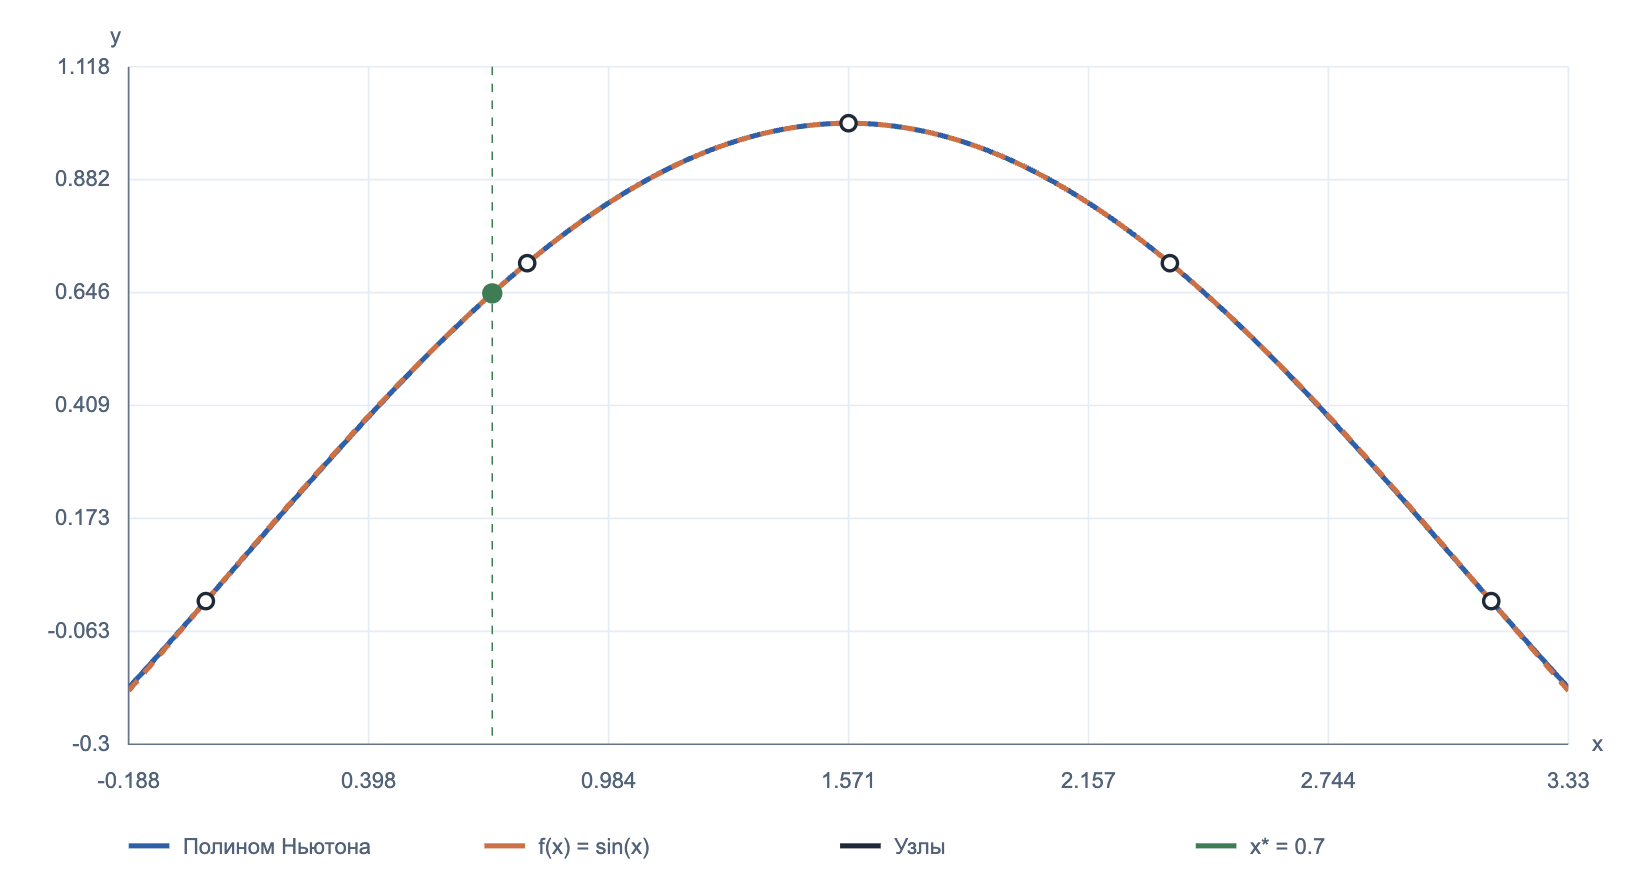
\includegraphics[width=\textwidth]{docs/graph-sin.png}
\caption{Интерполяция $\sin x$ по пяти узлам: функция и полином показаны разными цветами}
\end{figure}

\clearpage
\subsection{Веб-интерфейс}
Веб-интерфейс содержит левую панель ввода и правую область результатов.
Доступны редактирование узлов,
загрузка файлов, табулирование функции, выбор аргумента, просмотр разностей
и скачивание текстового результата или SVG. График поддерживает масштабирование
колесом и кнопками, перемещение перетаскиванием и сброс масштаба.

\begin{figure}[H]\centering
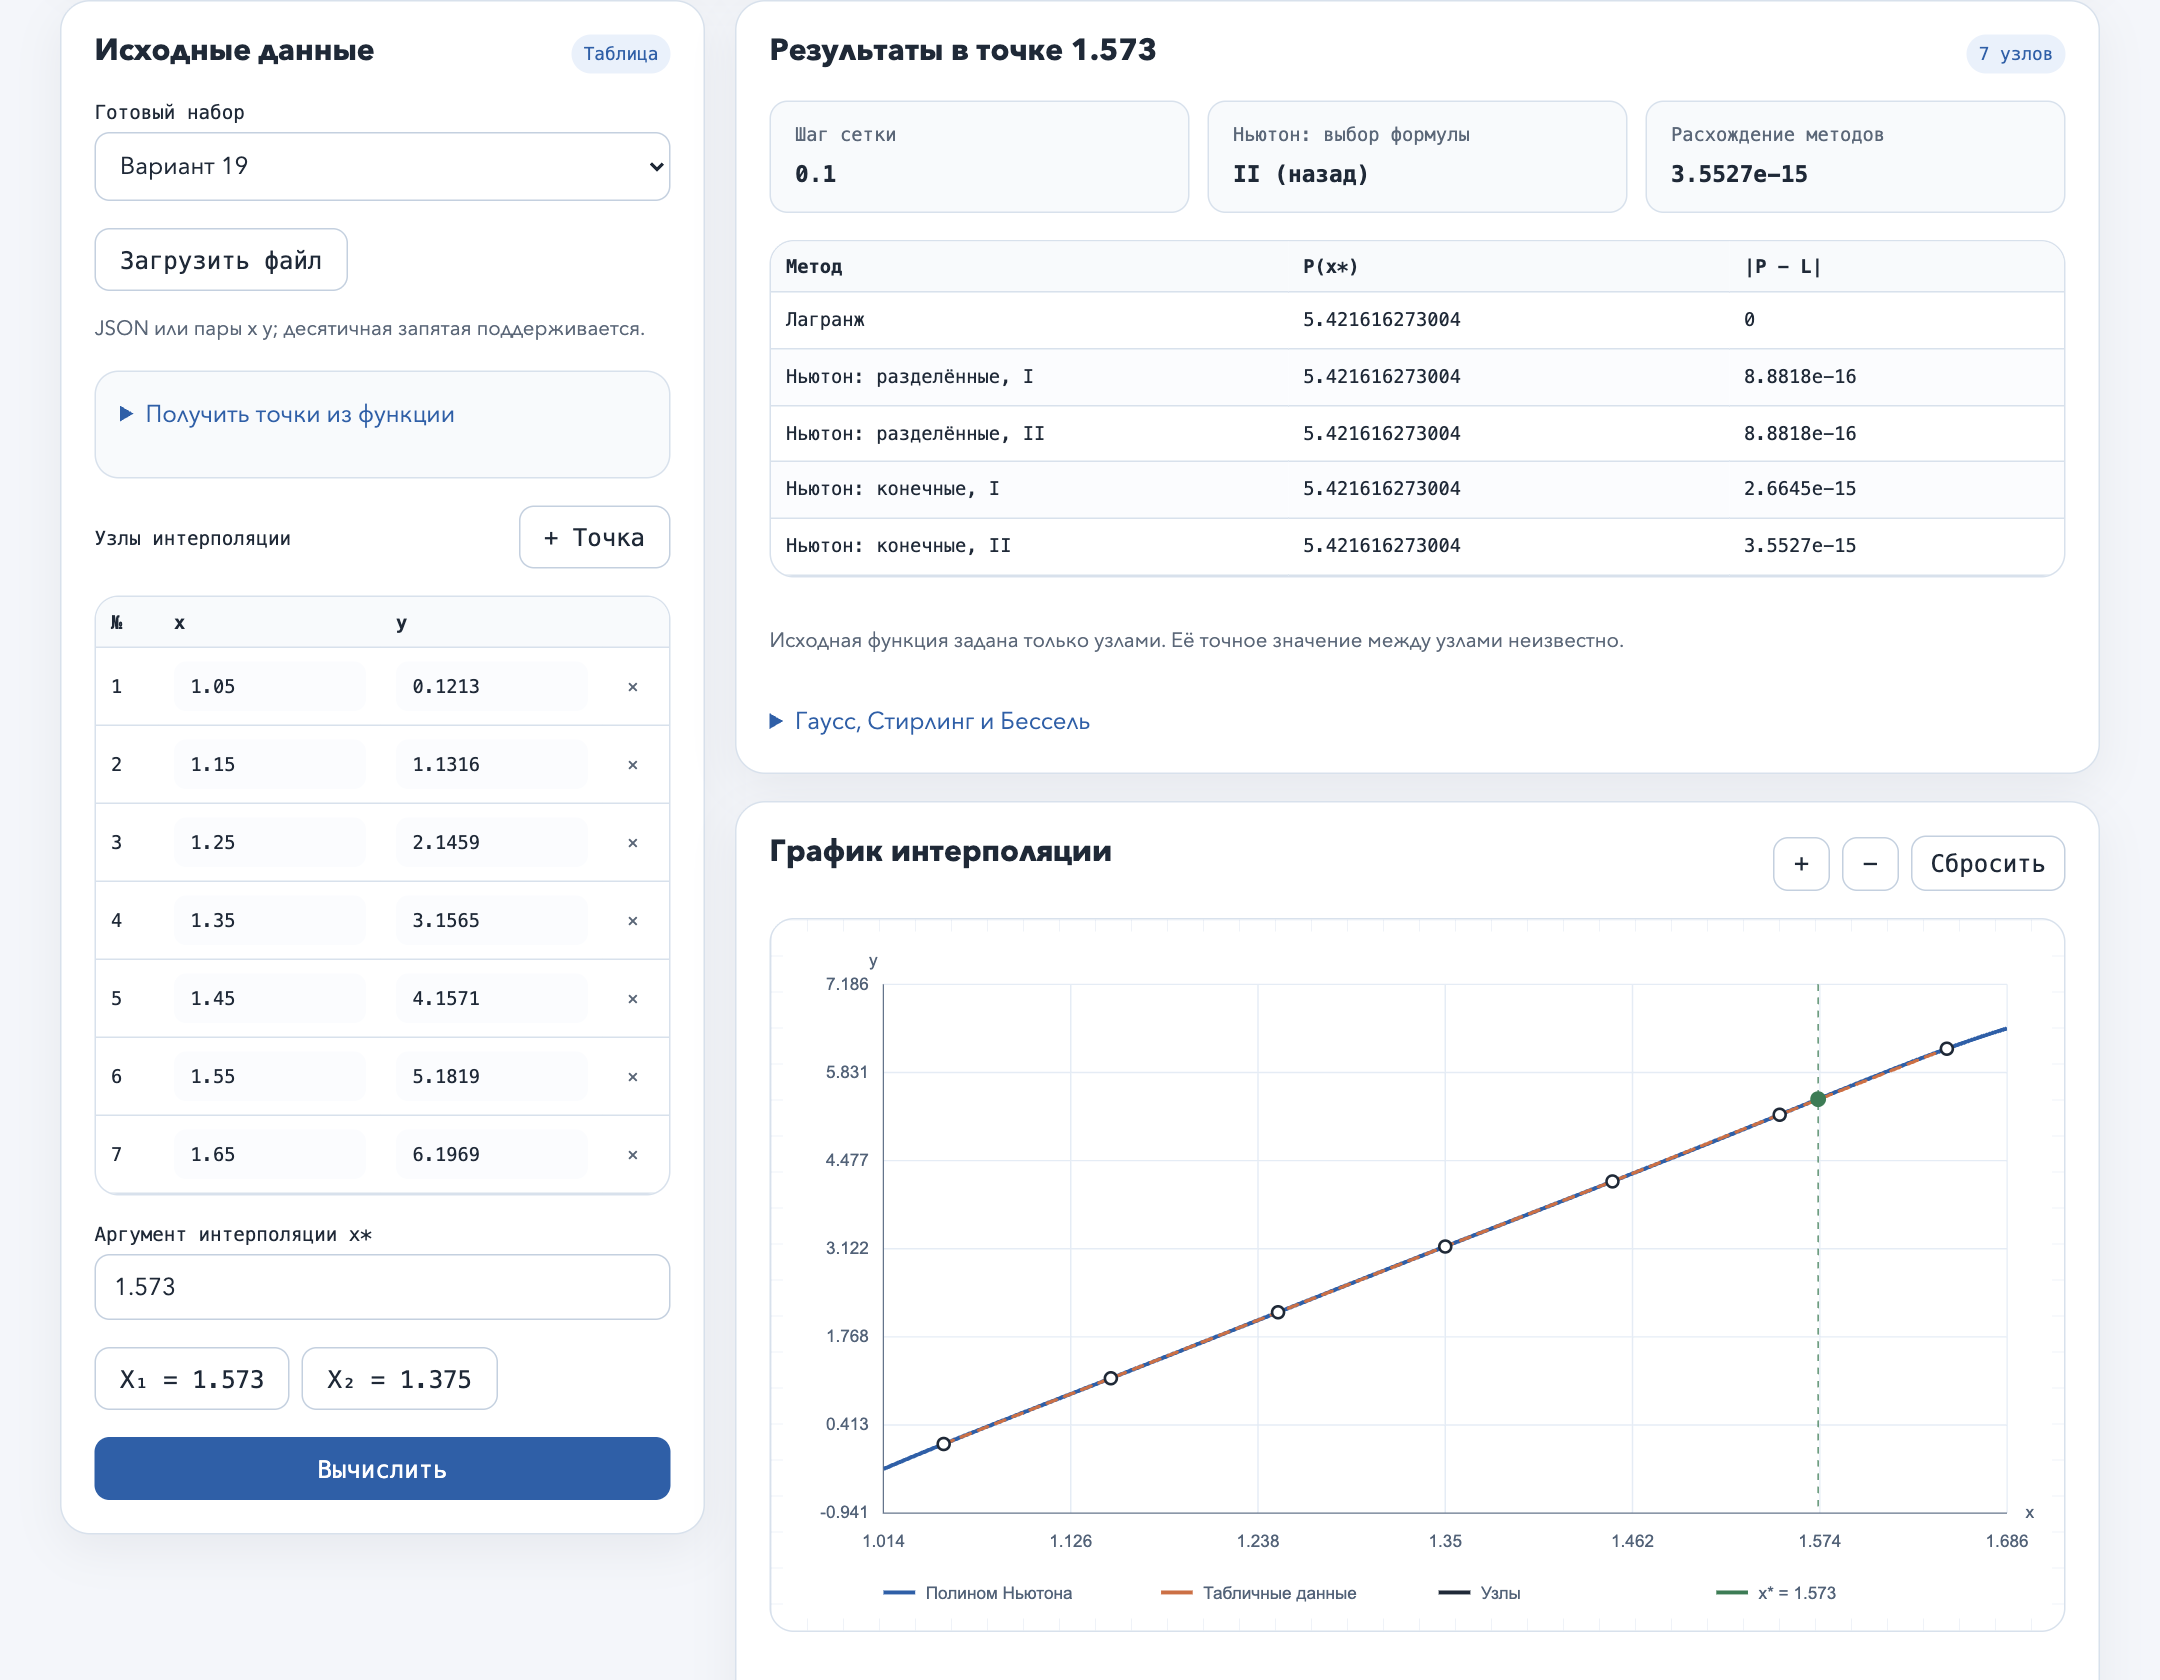
\includegraphics[width=\textwidth]{docs/screen-web-desktop-report.png}
\caption{Веб-интерфейс ЛР №5 в широком окне}
\end{figure}
\clearpage
\begin{figure}[H]\centering
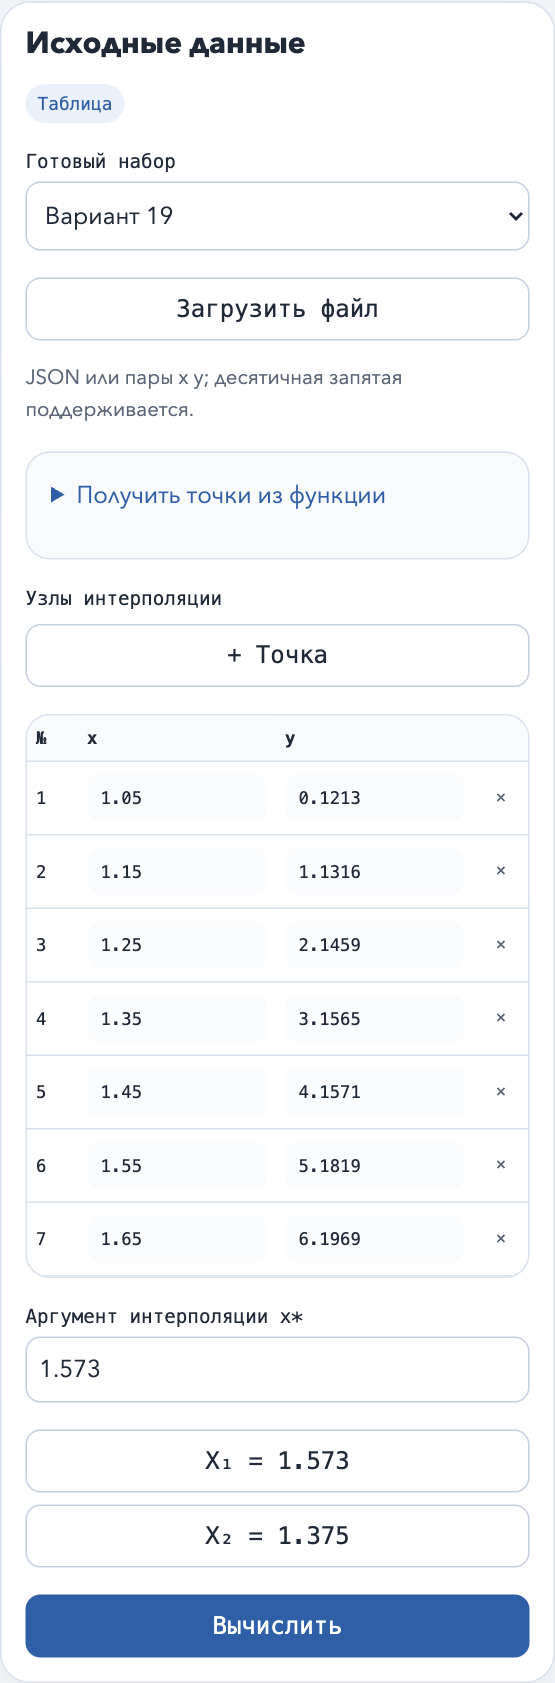
\includegraphics[width=0.62\textwidth,height=0.84\textheight,keepaspectratio]{docs/screen-web-mobile-report.png}
\caption{Адаптивная форма в окне шириной 390 пикселей}
\end{figure}

\clearpage
\subsection{Проверка программы}
Подготовлены четыре корректных JSON-набора, текстовый набор с десятичной
запятой и два некорректных файла.
\begin{table}[H]\centering\small
\caption{Контрольные наборы и фактические результаты}
\begin{tabular}{p{3.7cm}p{5cm}p{5cm}}\toprule
Набор & Проверка & Результат\\\midrule
Вариант 19 & 7 узлов, два аргумента & Совпадение с вычислительной частью\\
Неравномерная сетка & $y=x^2-2x+3$, $x=0.7$ & $2.09$; конечные схемы неприменимы\\
Кубический полином & 6 узлов, $x=0.25$ & $0.515625$, включая Бесселя\\
Синус & 7 узлов на $[0;\pi]$, $x=0.7$ & Сравнение с $\sin(0.7)$, вывод ошибки\\
Десятичная запятая & Текст с разделителем «;» & Успешное чтение чисел\\
Повторяющийся $x$ & Две точки с $x=0$ & Диагностика различных узлов\\
Одна точка & Недостаточный размер таблицы & Ошибка: требуется от 2 до 50 точек\\\bottomrule
\end{tabular}\end{table}

Все 21 автоматический тест завершились успешно. Проверяются значения варианта,
воспроизведение полиномов степеней 1--8, прохождение через каждый узел,
неравномерная сетка, сортировка, малые масштабы, форматы файлов,
нечисловые и бесконечные значения, повторяющиеся узлы, некорректные интервалы,
табулирование трёх функций, экстраполяция и работа консоли, включая ввод с клавиатуры.
Контрольные значения варианта дополнительно получены независимым расчётом
в рациональной арифметике.

В браузере проверены исходный расчёт, переход к $X_2$, изменение масштаба
и сброс, неравномерный набор, чётный набор для Бесселя, генерация функции,
диагностика повторяющихся узлов, загрузка файла и скачивание результата.
В окне 390 пикселей таблицы прокручиваются внутри своих блоков;
горизонтального переполнения страницы нет. Ошибок JavaScript не обнаружено.

\clearpage
\section{Вывод}
Для таблицы варианта 19 построены конечные разности до шестого порядка.
По второй формуле Ньютона получено $f(1.573)\approx5.421616273004$,
по первой формуле Гаусса --- $f(1.375)\approx3.406628713989$.
Многочлен Лагранжа дал те же значения; максимальное расхождение результатов
составило $3.55\cdot10^{-15}$. Программа выводит таблицы конечных и разделённых
разностей, вычисляет значения интерполяционного многочлена и строит его график.
Все 21 автоматический тест завершились без ошибок.
\end{document}
